% GNUPLOT: LaTeX picture with Postscript
\begingroup
  \makeatletter
  \providecommand\color[2][]{%
    \GenericError{(gnuplot) \space\space\space\@spaces}{%
      Package color not loaded in conjunction with
      terminal option `colourtext'%
    }{See the gnuplot documentation for explanation.%
    }{Either use 'blacktext' in gnuplot or load the package
      color.sty in LaTeX.}%
    \renewcommand\color[2][]{}%
  }%
  \providecommand\includegraphics[2][]{%
    \GenericError{(gnuplot) \space\space\space\@spaces}{%
      Package graphicx or graphics not loaded%
    }{See the gnuplot documentation for explanation.%
    }{The gnuplot epslatex terminal needs graphicx.sty or graphics.sty.}%
    \renewcommand\includegraphics[2][]{}%
  }%
  \providecommand\rotatebox[2]{#2}%
  \@ifundefined{ifGPcolor}{%
    \newif\ifGPcolor
    \GPcolortrue
  }{}%
  \@ifundefined{ifGPblacktext}{%
    \newif\ifGPblacktext
    \GPblacktexttrue
  }{}%
  % define a \g@addto@macro without @ in the name:
  \let\gplgaddtomacro\g@addto@macro
  % define empty templates for all commands taking text:
  \gdef\gplbacktext{}%
  \gdef\gplfronttext{}%
  \makeatother
  \ifGPblacktext
    % no textcolor at all
    \def\colorrgb#1{}%
    \def\colorgray#1{}%
  \else
    % gray or color?
    \ifGPcolor
      \def\colorrgb#1{\color[rgb]{#1}}%
      \def\colorgray#1{\color[gray]{#1}}%
      \expandafter\def\csname LTw\endcsname{\color{white}}%
      \expandafter\def\csname LTb\endcsname{\color{black}}%
      \expandafter\def\csname LTa\endcsname{\color{black}}%
      \expandafter\def\csname LT0\endcsname{\color[rgb]{1,0,0}}%
      \expandafter\def\csname LT1\endcsname{\color[rgb]{0,1,0}}%
      \expandafter\def\csname LT2\endcsname{\color[rgb]{0,0,1}}%
      \expandafter\def\csname LT3\endcsname{\color[rgb]{1,0,1}}%
      \expandafter\def\csname LT4\endcsname{\color[rgb]{0,1,1}}%
      \expandafter\def\csname LT5\endcsname{\color[rgb]{1,1,0}}%
      \expandafter\def\csname LT6\endcsname{\color[rgb]{0,0,0}}%
      \expandafter\def\csname LT7\endcsname{\color[rgb]{1,0.3,0}}%
      \expandafter\def\csname LT8\endcsname{\color[rgb]{0.5,0.5,0.5}}%
    \else
      % gray
      \def\colorrgb#1{\color{black}}%
      \def\colorgray#1{\color[gray]{#1}}%
      \expandafter\def\csname LTw\endcsname{\color{white}}%
      \expandafter\def\csname LTb\endcsname{\color{black}}%
      \expandafter\def\csname LTa\endcsname{\color{black}}%
      \expandafter\def\csname LT0\endcsname{\color{black}}%
      \expandafter\def\csname LT1\endcsname{\color{black}}%
      \expandafter\def\csname LT2\endcsname{\color{black}}%
      \expandafter\def\csname LT3\endcsname{\color{black}}%
      \expandafter\def\csname LT4\endcsname{\color{black}}%
      \expandafter\def\csname LT5\endcsname{\color{black}}%
      \expandafter\def\csname LT6\endcsname{\color{black}}%
      \expandafter\def\csname LT7\endcsname{\color{black}}%
      \expandafter\def\csname LT8\endcsname{\color{black}}%
    \fi
  \fi
    \setlength{\unitlength}{0.0500bp}%
    \ifx\gptboxheight\undefined%
      \newlength{\gptboxheight}%
      \newlength{\gptboxwidth}%
      \newsavebox{\gptboxtext}%
    \fi%
    \setlength{\fboxrule}{0.5pt}%
    \setlength{\fboxsep}{1pt}%
\begin{picture}(7920.00,5940.00)%
    \gplgaddtomacro\gplbacktext{%
      \csname LTb\endcsname%
      \put(831,4178){\makebox(0,0)[r]{\strut{}$10^{-3}$}}%
      \csname LTb\endcsname%
      \put(831,4398){\makebox(0,0)[r]{\strut{}$10^{-2}$}}%
      \csname LTb\endcsname%
      \put(831,4619){\makebox(0,0)[r]{\strut{}$10^{-1}$}}%
      \csname LTb\endcsname%
      \put(831,4839){\makebox(0,0)[r]{\strut{}$10^{0}$}}%
      \csname LTb\endcsname%
      \put(831,5059){\makebox(0,0)[r]{\strut{}$10^{1}$}}%
      \csname LTb\endcsname%
      \put(831,5279){\makebox(0,0)[r]{\strut{}$10^{2}$}}%
      \csname LTb\endcsname%
      \put(831,5500){\makebox(0,0)[r]{\strut{}$10^{3}$}}%
      \csname LTb\endcsname%
      \put(831,5720){\makebox(0,0)[r]{\strut{}$10^{4}$}}%
      \csname LTb\endcsname%
      \put(919,3979){\makebox(0,0){\strut{} }}%
      \csname LTb\endcsname%
      \put(1283,3979){\makebox(0,0){\strut{} }}%
      \csname LTb\endcsname%
      \put(1647,3979){\makebox(0,0){\strut{} }}%
      \csname LTb\endcsname%
      \put(2011,3979){\makebox(0,0){\strut{} }}%
      \csname LTb\endcsname%
      \put(2375,3979){\makebox(0,0){\strut{} }}%
      \csname LTb\endcsname%
      \put(2739,3979){\makebox(0,0){\strut{} }}%
      \csname LTb\endcsname%
      \put(3103,3979){\makebox(0,0){\strut{} }}%
      \csname LTb\endcsname%
      \put(3467,3979){\makebox(0,0){\strut{} }}%
      \csname LTb\endcsname%
      \put(3831,3979){\makebox(0,0){\strut{} }}%
      \csname LTb\endcsname%
      \put(3919,4178){\makebox(0,0)[l]{\strut{} }}%
      \csname LTb\endcsname%
      \put(3919,4398){\makebox(0,0)[l]{\strut{} }}%
      \csname LTb\endcsname%
      \put(3919,4619){\makebox(0,0)[l]{\strut{} }}%
      \csname LTb\endcsname%
      \put(3919,4839){\makebox(0,0)[l]{\strut{} }}%
      \csname LTb\endcsname%
      \put(3919,5059){\makebox(0,0)[l]{\strut{} }}%
      \csname LTb\endcsname%
      \put(3919,5279){\makebox(0,0)[l]{\strut{} }}%
      \csname LTb\endcsname%
      \put(3919,5500){\makebox(0,0)[l]{\strut{} }}%
      \csname LTb\endcsname%
      \put(3919,5720){\makebox(0,0)[l]{\strut{} }}%
      \csname LTb\endcsname%
      \put(919,5919){\makebox(0,0){\strut{}$10^{2}$}}%
      \csname LTb\endcsname%
      \put(1501,5919){\makebox(0,0){\strut{}$10^{3}$}}%
      \csname LTb\endcsname%
      \put(2084,5919){\makebox(0,0){\strut{}$10^{4}$}}%
      \csname LTb\endcsname%
      \put(2666,5919){\makebox(0,0){\strut{}$10^{5}$}}%
      \csname LTb\endcsname%
      \put(3249,5919){\makebox(0,0){\strut{}$10^{6}$}}%
      \csname LTb\endcsname%
      \put(3831,5919){\makebox(0,0){\strut{}$10^{7}$}}%
    }%
    \gplgaddtomacro\gplfronttext{%
      \csname LTb\endcsname%
      \put(291,4949){\rotatebox{-270}{\makebox(0,0){\strut{}$k = 2$}}}%
    }%
    \gplgaddtomacro\gplbacktext{%
      \csname LTb\endcsname%
      \put(3999,4178){\makebox(0,0)[r]{\strut{} }}%
      \csname LTb\endcsname%
      \put(3999,4398){\makebox(0,0)[r]{\strut{} }}%
      \csname LTb\endcsname%
      \put(3999,4619){\makebox(0,0)[r]{\strut{} }}%
      \csname LTb\endcsname%
      \put(3999,4839){\makebox(0,0)[r]{\strut{} }}%
      \csname LTb\endcsname%
      \put(3999,5059){\makebox(0,0)[r]{\strut{} }}%
      \csname LTb\endcsname%
      \put(3999,5279){\makebox(0,0)[r]{\strut{} }}%
      \csname LTb\endcsname%
      \put(3999,5500){\makebox(0,0)[r]{\strut{} }}%
      \csname LTb\endcsname%
      \put(3999,5720){\makebox(0,0)[r]{\strut{} }}%
      \csname LTb\endcsname%
      \put(4087,3979){\makebox(0,0){\strut{} }}%
      \csname LTb\endcsname%
      \put(4503,3979){\makebox(0,0){\strut{} }}%
      \csname LTb\endcsname%
      \put(4919,3979){\makebox(0,0){\strut{} }}%
      \csname LTb\endcsname%
      \put(5335,3979){\makebox(0,0){\strut{} }}%
      \csname LTb\endcsname%
      \put(5751,3979){\makebox(0,0){\strut{} }}%
      \csname LTb\endcsname%
      \put(6167,3979){\makebox(0,0){\strut{} }}%
      \csname LTb\endcsname%
      \put(6583,3979){\makebox(0,0){\strut{} }}%
      \csname LTb\endcsname%
      \put(6999,3979){\makebox(0,0){\strut{} }}%
      \csname LTb\endcsname%
      \put(7087,4178){\makebox(0,0)[l]{\strut{}$10^{-3}$}}%
      \csname LTb\endcsname%
      \put(7087,4398){\makebox(0,0)[l]{\strut{}$10^{-2}$}}%
      \csname LTb\endcsname%
      \put(7087,4619){\makebox(0,0)[l]{\strut{}$10^{-1}$}}%
      \csname LTb\endcsname%
      \put(7087,4839){\makebox(0,0)[l]{\strut{}$10^{0}$}}%
      \csname LTb\endcsname%
      \put(7087,5059){\makebox(0,0)[l]{\strut{}$10^{1}$}}%
      \csname LTb\endcsname%
      \put(7087,5279){\makebox(0,0)[l]{\strut{}$10^{2}$}}%
      \csname LTb\endcsname%
      \put(7087,5500){\makebox(0,0)[l]{\strut{}$10^{3}$}}%
      \csname LTb\endcsname%
      \put(7087,5720){\makebox(0,0)[l]{\strut{}$10^{4}$}}%
      \csname LTb\endcsname%
      \put(4087,5919){\makebox(0,0){\strut{}$10^{2}$}}%
      \csname LTb\endcsname%
      \put(4815,5919){\makebox(0,0){\strut{}$10^{3}$}}%
      \csname LTb\endcsname%
      \put(5543,5919){\makebox(0,0){\strut{}$10^{4}$}}%
      \csname LTb\endcsname%
      \put(6271,5919){\makebox(0,0){\strut{}$10^{5}$}}%
      \csname LTb\endcsname%
      \put(6999,5919){\makebox(0,0){\strut{}$10^{6}$}}%
    }%
    \gplgaddtomacro\gplfronttext{%
      \csname LTb\endcsname%
      \put(7625,4949){\rotatebox{-270}{\makebox(0,0){\strut{}$k = 3$}}}%
    }%
    \gplgaddtomacro\gplbacktext{%
      \csname LTb\endcsname%
      \put(831,2198){\makebox(0,0)[r]{\strut{}$10^{-3}$}}%
      \csname LTb\endcsname%
      \put(831,2418){\makebox(0,0)[r]{\strut{}$10^{-2}$}}%
      \csname LTb\endcsname%
      \put(831,2639){\makebox(0,0)[r]{\strut{}$10^{-1}$}}%
      \csname LTb\endcsname%
      \put(831,2859){\makebox(0,0)[r]{\strut{}$10^{0}$}}%
      \csname LTb\endcsname%
      \put(831,3080){\makebox(0,0)[r]{\strut{}$10^{1}$}}%
      \csname LTb\endcsname%
      \put(831,3300){\makebox(0,0)[r]{\strut{}$10^{2}$}}%
      \csname LTb\endcsname%
      \put(831,3521){\makebox(0,0)[r]{\strut{}$10^{3}$}}%
      \csname LTb\endcsname%
      \put(831,3741){\makebox(0,0)[r]{\strut{}$10^{4}$}}%
      \csname LTb\endcsname%
      \put(919,1999){\makebox(0,0){\strut{} }}%
      \csname LTb\endcsname%
      \put(1890,1999){\makebox(0,0){\strut{} }}%
      \csname LTb\endcsname%
      \put(2860,1999){\makebox(0,0){\strut{} }}%
      \csname LTb\endcsname%
      \put(3831,1999){\makebox(0,0){\strut{} }}%
      \csname LTb\endcsname%
      \put(3919,2198){\makebox(0,0)[l]{\strut{} }}%
      \csname LTb\endcsname%
      \put(3919,2418){\makebox(0,0)[l]{\strut{} }}%
      \csname LTb\endcsname%
      \put(3919,2639){\makebox(0,0)[l]{\strut{} }}%
      \csname LTb\endcsname%
      \put(3919,2859){\makebox(0,0)[l]{\strut{} }}%
      \csname LTb\endcsname%
      \put(3919,3080){\makebox(0,0)[l]{\strut{} }}%
      \csname LTb\endcsname%
      \put(3919,3300){\makebox(0,0)[l]{\strut{} }}%
      \csname LTb\endcsname%
      \put(3919,3521){\makebox(0,0)[l]{\strut{} }}%
      \csname LTb\endcsname%
      \put(3919,3741){\makebox(0,0)[l]{\strut{} }}%
      \csname LTb\endcsname%
      \put(919,3940){\makebox(0,0){\strut{} }}%
      \csname LTb\endcsname%
      \put(1404,3940){\makebox(0,0){\strut{} }}%
      \csname LTb\endcsname%
      \put(1890,3940){\makebox(0,0){\strut{} }}%
      \csname LTb\endcsname%
      \put(2375,3940){\makebox(0,0){\strut{} }}%
      \csname LTb\endcsname%
      \put(2860,3940){\makebox(0,0){\strut{} }}%
      \csname LTb\endcsname%
      \put(3346,3940){\makebox(0,0){\strut{} }}%
      \csname LTb\endcsname%
      \put(3831,3940){\makebox(0,0){\strut{} }}%
    }%
    \gplgaddtomacro\gplfronttext{%
      \csname LTb\endcsname%
      \put(291,2969){\rotatebox{-270}{\makebox(0,0){\strut{}$k = 4$}}}%
    }%
    \gplgaddtomacro\gplbacktext{%
      \csname LTb\endcsname%
      \put(3999,2198){\makebox(0,0)[r]{\strut{} }}%
      \csname LTb\endcsname%
      \put(3999,2418){\makebox(0,0)[r]{\strut{} }}%
      \csname LTb\endcsname%
      \put(3999,2639){\makebox(0,0)[r]{\strut{} }}%
      \csname LTb\endcsname%
      \put(3999,2859){\makebox(0,0)[r]{\strut{} }}%
      \csname LTb\endcsname%
      \put(3999,3080){\makebox(0,0)[r]{\strut{} }}%
      \csname LTb\endcsname%
      \put(3999,3300){\makebox(0,0)[r]{\strut{} }}%
      \csname LTb\endcsname%
      \put(3999,3521){\makebox(0,0)[r]{\strut{} }}%
      \csname LTb\endcsname%
      \put(3999,3741){\makebox(0,0)[r]{\strut{} }}%
      \csname LTb\endcsname%
      \put(4087,1999){\makebox(0,0){\strut{}$10^{3}$}}%
      \csname LTb\endcsname%
      \put(5058,1999){\makebox(0,0){\strut{}$10^{4}$}}%
      \csname LTb\endcsname%
      \put(6028,1999){\makebox(0,0){\strut{}$10^{5}$}}%
      \csname LTb\endcsname%
      \put(6999,1999){\makebox(0,0){\strut{}$10^{6}$}}%
      \csname LTb\endcsname%
      \put(7087,2198){\makebox(0,0)[l]{\strut{}$10^{-3}$}}%
      \csname LTb\endcsname%
      \put(7087,2418){\makebox(0,0)[l]{\strut{}$10^{-2}$}}%
      \csname LTb\endcsname%
      \put(7087,2639){\makebox(0,0)[l]{\strut{}$10^{-1}$}}%
      \csname LTb\endcsname%
      \put(7087,2859){\makebox(0,0)[l]{\strut{}$10^{0}$}}%
      \csname LTb\endcsname%
      \put(7087,3080){\makebox(0,0)[l]{\strut{}$10^{1}$}}%
      \csname LTb\endcsname%
      \put(7087,3300){\makebox(0,0)[l]{\strut{}$10^{2}$}}%
      \csname LTb\endcsname%
      \put(7087,3521){\makebox(0,0)[l]{\strut{}$10^{3}$}}%
      \csname LTb\endcsname%
      \put(7087,3741){\makebox(0,0)[l]{\strut{}$10^{4}$}}%
      \csname LTb\endcsname%
      \put(4087,3940){\makebox(0,0){\strut{} }}%
      \csname LTb\endcsname%
      \put(4378,3940){\makebox(0,0){\strut{} }}%
      \csname LTb\endcsname%
      \put(4669,3940){\makebox(0,0){\strut{} }}%
      \csname LTb\endcsname%
      \put(4961,3940){\makebox(0,0){\strut{} }}%
      \csname LTb\endcsname%
      \put(5252,3940){\makebox(0,0){\strut{} }}%
      \csname LTb\endcsname%
      \put(5543,3940){\makebox(0,0){\strut{} }}%
      \csname LTb\endcsname%
      \put(5834,3940){\makebox(0,0){\strut{} }}%
      \csname LTb\endcsname%
      \put(6125,3940){\makebox(0,0){\strut{} }}%
      \csname LTb\endcsname%
      \put(6417,3940){\makebox(0,0){\strut{} }}%
      \csname LTb\endcsname%
      \put(6708,3940){\makebox(0,0){\strut{} }}%
      \csname LTb\endcsname%
      \put(6999,3940){\makebox(0,0){\strut{} }}%
    }%
    \gplgaddtomacro\gplfronttext{%
      \csname LTb\endcsname%
      \put(7625,2969){\rotatebox{-270}{\makebox(0,0){\strut{}$k = 5$}}}%
    }%
    \gplgaddtomacro\gplbacktext{%
      \csname LTb\endcsname%
      \put(831,218){\makebox(0,0)[r]{\strut{}$10^{-3}$}}%
      \csname LTb\endcsname%
      \put(831,438){\makebox(0,0)[r]{\strut{}$10^{-2}$}}%
      \csname LTb\endcsname%
      \put(831,659){\makebox(0,0)[r]{\strut{}$10^{-1}$}}%
      \csname LTb\endcsname%
      \put(831,879){\makebox(0,0)[r]{\strut{}$10^{0}$}}%
      \csname LTb\endcsname%
      \put(831,1100){\makebox(0,0)[r]{\strut{}$10^{1}$}}%
      \csname LTb\endcsname%
      \put(831,1320){\makebox(0,0)[r]{\strut{}$10^{2}$}}%
      \csname LTb\endcsname%
      \put(831,1541){\makebox(0,0)[r]{\strut{}$10^{3}$}}%
      \csname LTb\endcsname%
      \put(831,1761){\makebox(0,0)[r]{\strut{}$10^{4}$}}%
      \csname LTb\endcsname%
      \put(919,19){\makebox(0,0){\strut{}$10^{3}$}}%
      \csname LTb\endcsname%
      \put(1890,19){\makebox(0,0){\strut{}$10^{4}$}}%
      \csname LTb\endcsname%
      \put(2860,19){\makebox(0,0){\strut{}$10^{5}$}}%
      \csname LTb\endcsname%
      \put(3831,19){\makebox(0,0){\strut{}$10^{6}$}}%
      \csname LTb\endcsname%
      \put(3919,218){\makebox(0,0)[l]{\strut{} }}%
      \csname LTb\endcsname%
      \put(3919,438){\makebox(0,0)[l]{\strut{} }}%
      \csname LTb\endcsname%
      \put(3919,659){\makebox(0,0)[l]{\strut{} }}%
      \csname LTb\endcsname%
      \put(3919,879){\makebox(0,0)[l]{\strut{} }}%
      \csname LTb\endcsname%
      \put(3919,1100){\makebox(0,0)[l]{\strut{} }}%
      \csname LTb\endcsname%
      \put(3919,1320){\makebox(0,0)[l]{\strut{} }}%
      \csname LTb\endcsname%
      \put(3919,1541){\makebox(0,0)[l]{\strut{} }}%
      \csname LTb\endcsname%
      \put(3919,1761){\makebox(0,0)[l]{\strut{} }}%
      \csname LTb\endcsname%
      \put(919,1960){\makebox(0,0){\strut{} }}%
      \csname LTb\endcsname%
      \put(1210,1960){\makebox(0,0){\strut{} }}%
      \csname LTb\endcsname%
      \put(1501,1960){\makebox(0,0){\strut{} }}%
      \csname LTb\endcsname%
      \put(1793,1960){\makebox(0,0){\strut{} }}%
      \csname LTb\endcsname%
      \put(2084,1960){\makebox(0,0){\strut{} }}%
      \csname LTb\endcsname%
      \put(2375,1960){\makebox(0,0){\strut{} }}%
      \csname LTb\endcsname%
      \put(2666,1960){\makebox(0,0){\strut{} }}%
      \csname LTb\endcsname%
      \put(2957,1960){\makebox(0,0){\strut{} }}%
      \csname LTb\endcsname%
      \put(3249,1960){\makebox(0,0){\strut{} }}%
      \csname LTb\endcsname%
      \put(3540,1960){\makebox(0,0){\strut{} }}%
      \csname LTb\endcsname%
      \put(3831,1960){\makebox(0,0){\strut{} }}%
    }%
    \gplgaddtomacro\gplfronttext{%
      \csname LTb\endcsname%
      \put(291,989){\rotatebox{-270}{\makebox(0,0){\strut{}$k = 6$}}}%
      \csname LTb\endcsname%
      \put(3224,1661){\makebox(0,0)[r]{\strut{}Pardiso}}%
      \csname LTb\endcsname%
      \put(3224,1462){\makebox(0,0)[r]{\strut{}Mumps}}%
    }%
    \gplbacktext
    \put(0,0){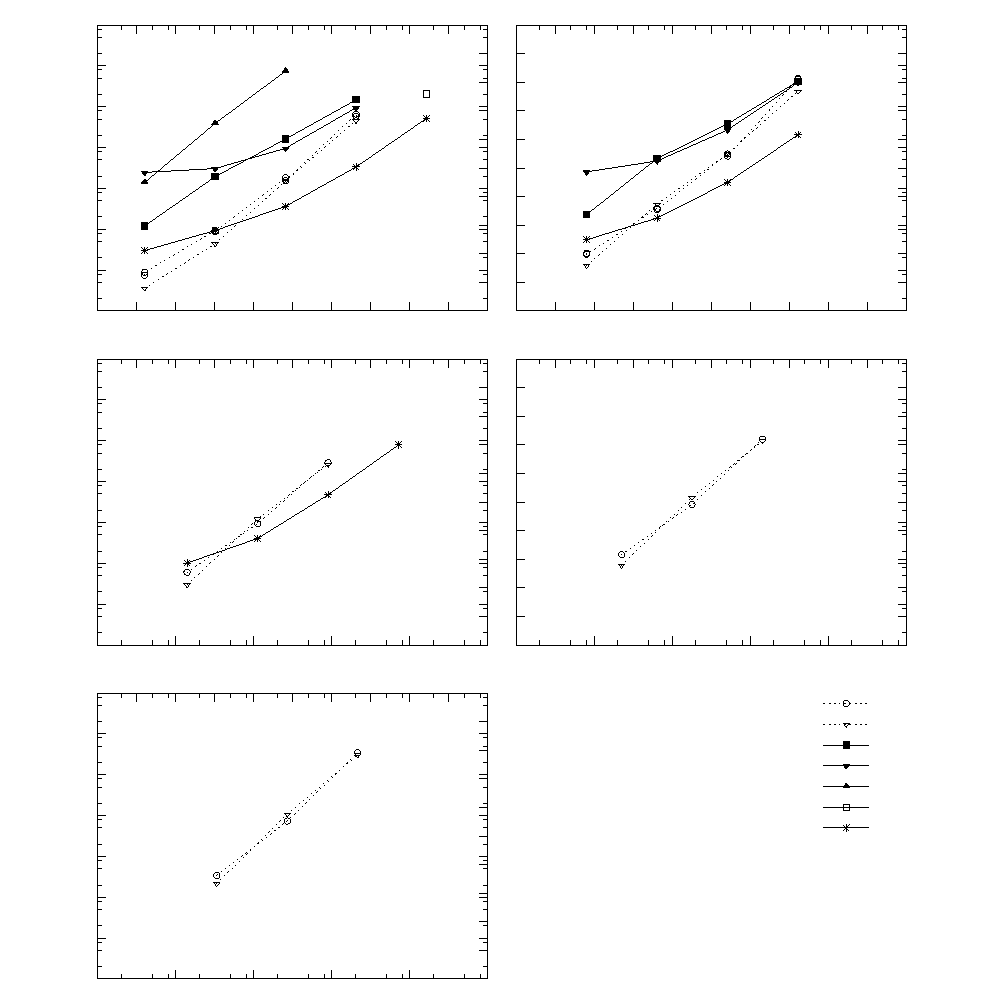
\includegraphics{ConstCoeffPoissonScaling}}%
    \gplfronttext
  \end{picture}%
\endgroup
